\subsection{Vorbereitung}
Bevor der eigentliche Versuch beginnt, werden für drei periodische Funktionen
die jeweiligen Fourier-Koeffizienten berechnet.
% Für periodische Funktionen besagt das Fouriersche Theorem, dass sie sich durch
% sinus- und cosinus-Funktionen nach der Formel
% \begin{equation}
%   f(t)= \frac{a_0}{2} + \sum_{n=1}^\infty \Biggl(a_n \cdot \cos \biggl(\frac{2n\pi t}{T} \biggr) + b_n \cdot \sin \biggl(\frac{2n\pi t}{T}\biggr)\Biggr)
% \end{equation}
% darstellen lassen. Dazu muss die Reihe jedoch konvergieren, mit ganzzahligem $n$. Die Parameter $a_n$ und $b_n$
% lassen sich dabei durch
% \begin{align}
%   a_n &= \frac{2}{T} \int_0^T f(t) \cdot \cos \biggl(\frac{2n\pi t}{T}\biggr) dt \\
%   b_n &= \frac{2}{T} \int_0^T f(t) \cdot \sin \biggl(\frac{2n\pi t}{T}\biggr) dt
% \end{align}
% bestimmen.
Bei den hier verwendeten Funktionen handelt es
sich um Rechteckspannung, Sägezahnspannung und Dreieckspannung. Zur Vereinfachung
werden diese so parametrisiert, dass sie entweder gerade oder ungerade sind.
Diese Vereinfachung führt dazu, dass bei geraden Funktionen $b_\su{n}=0$ und bei
ungeraden Funktionen $a_\su{n}=0$ für alle $n$ gilt.
\par
\noindent Die Vorbereitung wird mit den Formeln \eqref{theorem} und \eqref{eq:analyse} durchgeführt.
Für die Rechteckspannung ergibt sich
\[f_\su{recht}(t)=\begin{cases}
-1 & \text{für}\, -\pi<t<\pi\\
0 & \text{für}\, t=-\pi,0,\pi\\
1 &\text{für}\,  0<t<\pi \\
\end{cases}\]
Für gerade $n$ gilt $b_\su{n} = 0$ und für ungerade $n$ gilt $b_\su{n} = \frac{4}{n\pi}$.
\par
\noindent Bei der Sägezahnspannung folgt
\[f_\su{saege}(t)=\begin{cases}
t & \text{für}\,\, -\pi<t<\pi\\
0 & \text{für}\,\, t=-\pi,\pi\\
\end{cases}\]
mit $b_\su{n} = -\frac{2}{n}(-1)^{n+1}$.
\par
\noindent Für die Dreieckspannung ergibt sich
\begin{equation}
  f_\su{dreieck}(t) = |t|
\end{equation}
mit $a_\su{n} = 0$ für ungerade $n$ und $a_\su{n} = -\frac{4}{n^2\pi}$ für gerade $n$.
\par
\noindent Für die Rechteckspannung und die Sägezahnspannung ergeben sich damit die Zusammenhänge
von $\sfrac{1}{n}$, für die Dreieckspannung ergibt sich $\sfrac{1}{n^2}$.
\subsection{Fourier-Synthese}
Für die Fourier-Synthese werden zunächst zwei Ausgänge des Oberwellengenerators
an das Oszilloskop angeschlossen. Damit alle Ausgänge in Phase geschalten werden
können, wird das Oszilloskop zunächst in den X-Y-Betrieb geschaltet. Um eine
optimale Genauigkeit zu erhalten, werden die einzelnen Amplituden der Oberwellen
auf maximal eingestellt. Nun werden die Phasen so lange variiert, bis sich
Lissajous-Figuren, wie beispielsweise in Abbildung \ref{lissa}, bilden.
\begin{figure}[H]
  \centering
  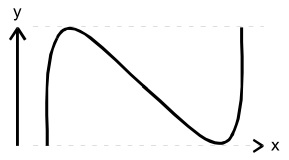
\includegraphics{bilder/lissajous.jpg}
  \caption{Beispiel für eine Lissajous-Figur}
  \label{lissa}
\end{figure}
% Wie es sich in der Vorbereitung
% herausgestellt hat, fallen die Koeffizienten der Funktionen der
% Sägezahn- und Recht-
% eckspannung mit dem Proportionalitätsfaktor X ab.
Die Ausgänge des Oszilloskops werden nun nacheinander an ein Voltmeter
angeschlossen. Die Amplituden der Oberwellen werden entsprechend eingestellt.
Das Oszilloskop wird in den normalen Betrieb zurückgeschaltet und der Generator
an das Oszilloskop angeschlossen. Die einzelnen Oberwellen werden aufaddiert und
gegebenenfalls in der Phase verschoben, bis möglichst genau eine Sägezahnspannung
approximiert wird.
Für die Rechteckspannung wird ähnlich vorgegangen, nur dass jetzt nur die
ungeraden Oberwellen benutzt werden.

Abschließend wird die Durchführung für die Dreieckspannung wiederholt. Hier müssen
zunächst die Amplituden mit dem Proportionalitätsfaktor X eingestellt werden.
Auch hier werden, wie bei der Rechteckspannung, nur die ungeraden Oberwellen
genutzt. Die Phase wird wieder so verschoben, dass die Dreieckspannung möglichst
genau approximiert wird.
\subsection{Fourier-Analyse}
Für die Fourier-Analyse von periodischen Schwingungen wird eine Schaltung wie in
Abbildung \ref{fig:ana} verwendet.
\begin{figure}[h]
  \centering
  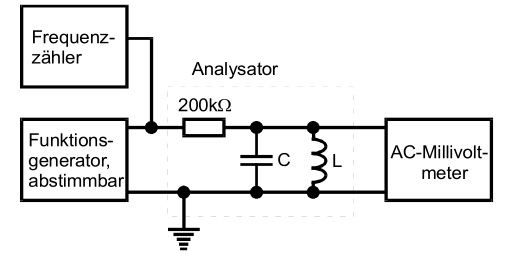
\includegraphics[width=0.8\textwidth]{bilder/analyse.jpg}
  \caption{Schaltung zur Fourier-Analyse\,\cite{351}}
  \label{fig:ana}
\end{figure}
Als Signalquelle dient hier ein durchstimmbarer Funktionsgenerator. Die
Transformation wird direkt vom Oszilloskop durchgeführt.

Damit genügend Peaks des Linienspektrums sichtbar werden, müssen ausreichend
Perioden angezeigt werden. Die angezeigten Peaks werden nun mit einer
Sinusspannung kalibriert und die Frequenz und die Amplitude werden notiert.
Nebenmaxima die sich bilden können, werden nicht beachtet. Die Messung wird für
alle genannten Funktionen durchgeführt.
